\chapter{Proof-Of-Concept Implementierung}
\label{ch:implementierung}


\section{FZ 1.3 Implementierung zur Vorverarbeitung medizinischer Texte}
\label{sec:FZ1.3} 

Da die zu verarbeitenden medizinischen Texte nicht nur Fließtext enthalten, sondern auch Überschriften und Aufzählungen, ist als erster Schritt eine sinnvolle Unterteilung in Satzeinheiten erforderlich. Dazu kommt die Bibliothek pySBD (\cite{sadvilkar_pysbd_2020}) zum Einsatz. Anschließend werden die Satzeinheiten noch so bearbeitet und zusammengefügt, dass möglichst sinnvolle Sätze für die weitere Verarbeitung entstehen. Ist eine erkannte Satzeinheit zum Beispiel ein leerer String, so wird diese nicht weiter verarbeitet. Nachgestellte Leerzeichen werden gelöscht. Außerdem werden Aufzählungen möglichst in einzelne Sätze verwandelt. So wird beispielsweise aus der Auflistung\\
\begin{addmargin}{10pt}
\emph{
	The psychological symptoms of depression include:\\
	- continuous low mood or sadness\\
	- feeling hopeless and helpless\\
	- having low self-esteem
}
\end{addmargin}
\vspace*{5mm}
eine Reihe von Sätzen:\\
\begin{addmargin}{10pt}
\emph{
	The psychological symptoms of depression include continuous low mood or sadness.\\
	The psychological symptoms of depression include feeling hopeless and helpless.\\
	The psychological symptoms of depression include having low self-esteem.
}
\end{addmargin}
\vspace*{5mm}
\section[FZ 2.4 Implementierung zur Überf. med. Fachvokabulars]{FZ 2.4 Implementierung zur Überführung medizinischen Fachvokabulars in maschinenlesbare Form zur weiteren Verarbeitung durch NLP}
\label{sec:FZ2.4}

Wie in Abschnitt \ref{loesungsansatz} beschrieben, wurde das Vokabular der Datei \emph{postings} des MetaMapLite-Projektes verwendet. Aus dieser Datei wurden zwei Dateien \emph{training\_diseases\_original.txt} und \emph{training\_symptoms\_original.txt} extrahiert, die jeweils nur die Einträge enthalten, die in der \emph{postings}-Datei als \emph{disease} bzw. \emph{disorder} oder \emph{finding} markiert sind. Diese Dateien bleiben als Referenz unverändert. Das Programm verwendet Kopien namens \emph{training\_diseases\_working.txt} und \emph{training\_symptoms\_working.txt}, aus denen bei Bedarf Begriffe entfernt werden können. Dies ist sinnvoll, da die Vokabular-Dateien sehr umfangreich sind, dadurch aber auch Einträge enthalten, die zum Auffinden von Krankheiten und Symptomen nicht hilfreich sind.

Jeder Eintrag besteht aus dem CUI, der Krankheit bzw. dem Symptom und der Kategorisierung als \emph{DISEASE} oder \emph{FINDING}. Als Beispiel seien hier die Einträge für die Begriffe \emph{depression} und \emph{loss of interest} angegeben:

\begin{center}
\begin{tabular}{llll}
C0011570 & depression & DISEASE \\
C0424091 & loss of interest & FINDING \\
\end{tabular}
\end{center}

Für das Auffinden der Named Entities wird die \emph{spaCy}-Komponente \emph{Entity Ruler} verwendet. Diese durchsucht einen Text konventionell nach den in den beiden Vokabular-Dateien eingetragenen Begriffen und gibt im Fall von Mehrdeutigkeiten die jeweils längsten Begriffe aus. Der \emph{Entity Ruler} wird dem \emph{Entity Recognizer} vorgezogen, da letzterer auf statistischer Modellierung beruht und das spezifische medizinische Vokabular durch eine Vielzahl von Beispielsätzen trainiert werden muss. Da das Vokabular sehr umfangreich ist und Trainingssätze für das Vokabular (noch) nicht zur Verfügung stehen, kann der \emph{Entity Recognizer} nicht zuverlässig verwendet werden.

Die Verwendung des \emph{Entity Rulers} erfolgt im Modul \emph{knowledge\_extractor.py}. Der \emph{Entity Ruler} wird bei Instanziierung des \emph{KnowledgeExtractor}-Objektes trainiert, indem im Konstruktor zunächst die Vokabular-Dateien geladen, ihre Einträge aufbereitet und diese schließlich dem \emph{Entity Ruler} durch die \emph{spaCy}-Funktion \emph{add\_patterns()} übergeben werden. Ebenfalls im Konstruktor der \emph{KnowledgeExtractor}-Klasse wird ein \emph{KnowledgeBase}-Objekt erzeugt. Dieses dient dazu, gefundene Wissensinhalte zu speichern.

Die Suche nach Wissensinhalten ist in diesem Prototypen sehr einfach gehalten. Es wird in jedem vorprozessiertem Satz nach Entitäten (Krankheiten, Symptome) gesucht und eine Beziehung zwischen Krankheit und Symptom dann angenommen, wenn beide Begriffe in einem Satz vorkommen. Wird z.B. dem \emph{KnowledgeExtractor} der Satz \emph{\glqq During a period of depression, your symptoms may include loss of interest in everyday activities\flqq} übergeben, so findet der \emph{Entity Ruler} die Krankheit \emph{depression} und das Symptom \emph{loss of interest}. Der \emph{KnowledgeExtractor} sieht dann im Verlust von Interesse ein Symptom für eine Depression.

Symptome sind in der Vokabular-Datei nicht mit ihren Negationen enthalten. So gibt es z.B. in dem Symptom-Vokabular den Eintrag \emph{motivation}, aber nicht den Eintrag \emph{no motivation}. Aus dem Satz \emph{\glqq The psychological symptoms of depression include having no motivation or interest in things.\flqq} würde der KnowledgeExtractor daher den Zusammenhang extrahieren, dass \emph{motivation} ein Symptom von \emph{depression} ist. Um solche Fehler zu vermeiden, prüft der \emph{KnowledgeExtractor} für jedes gefundene Symptom, ob dessen Negierung, hier also \emph{no motivation}, in dem zu analysierenden Text enthalten ist. Ist dies der Fall, so speichert er die Negierung der gefundenen Entität in der Wissensbasis.

Allerdings funktioniert dieses einfache Konzept für obigen Beispielsatz nicht bei dem Symptom \emph{interest}, da vor diesem das Wort \emph{no} fehlt und aus dem Kontext erschlossen werden muss. Im \emph{spaCy Universe} (https://spacy.io/universe) gibt es das Projekt \emph{negspaCy}, das negierte Begriffe mit einem entsprechenden Tag versieht. Leider funktioniert dieses Modul nur für einfache Sätze und liefert bei den von uns untersuchten Beispieltexten zu häufig keine guten Ergebnisse. Daher wurde auf die Verwendung von \emph{negspaCy} verzichtet.

\section{FZ 3.3 Implementierung zur Wissensrepräsentation}
\label{sec:FZ3.3} 

\section{Implementierung weiterer Funktionalität}

Zusätzlich zu den ausgearbeiteten Forschungszielen haben sich während der Implementierung die folgenden Funktionalitäten herauskristallisiert, die einen Mehrwert für das Programm darstellen.

\subsection{Erstellung von Trainingsdaten für den Entity-Linker}

Analysiert der \emph{KnowledgeExtractor} zahlreiche Texte, so ergibt sich die Möglichkeit, nicht nur eine Wissensrepräsentation zu erstellen, sondern auch Beispielsätze zu sammeln. Der \emph{KnowledgeExtractor} speichert daher auch Beispielsätze in der Wissensbasis. Diese Beispielsätze können für das Training statistischer Modelle wie z.B. des \emph{Entity Linkers}, einer weiteren optionalen Komponente der \emph{spaCy}-Pipeline, eingesetzt werden.

Der \emph{Entity Linker} arbeitet zusammen mit dem \emph{Entity Ruler} bzw. \emph{Entity Recognizer} und verknüpft von diesen Komponenten gefundene Entitäten mit Entitäten aus seiner eigenen Wissensbasis. Die Idee des \emph{Entity Linkers} ist es, mehrdeutigen Entitäten (z.B. \emph{Apple}) kontextbezogen konkrete Entitäten zuzuordnen, also etwa die Frucht, die Firma \emph{Apple} oder die Stadt New York (\emph{Big Apple}). Die vom \emph{Entity Recognizer} oder \emph{Entity Ruler} gefundenen Begriffe werden in diesem Zusammenhang als \emph{Aliase} bezeichnet.

Der \emph{Entity Linker} kann somit auch dafür verwendet werden, Symptomen mögliche Krankheiten zuzuordnen, denn Symptome können zu mehreren Krankheiten gehören. Es wurde daher eine Funktion implementiert, den Inhalt der Wissensbasis des \emph{MedExtractors} in eine xml-Datei zu exportieren, in der die Daten so aufbereitet sind, dass sie einfach vom \emph{Entity Linker} importiert werden können. Wie dieser Import funktioniert, wird in dem Jupyter-Notebook \emph{entity\_linker\_demo.ipynb} vorgeführt.

Abbildung \ref{fig:jupyter} zeigt einen Ausschnitt aus diesem Jupyter Notebook. Der \emph{spaCy}-Pipeline wird ein Text übergeben, in dem ein Patient seine Beschwerden während des Besuchs einer Shopping Mall beschreibt. In den nächsten beiden Zeilen wird jeweils über die vom \emph{Entity Ruler} gefundenen Entitäten in der Liste \emph{doc.ents} iteriert. Der \emph{Entity Linker} besitzt als Attribut das \emph{spacy.KnowledgeBase}-Objekt \emph{kb}\footnote{die dazugehörige \emph{spaCy}-Klasse entspricht nicht der \emph{KnowledgeBase}-Klasse im Modul \emph{base.py} des \emph{Medextractors}}, in dem die vom Medextractor gefundenen Entitäten und Aliase mitsamt der Verknüpfungen (Links) zwischen Entitäten und Aliasen gespeichert sind (nicht jedoch die Beispielsätze). Im ersten Fall wird die Funktion \emph{get\_alias\_condidates()} des \emph{KnowledgeBase}-Objektes verwendet, um sich für jedes im Text gefundene Symptom die dazu verknüpften Krankheiten anzeigen zu lassen.

\begin{figure}[h]
    \centering
    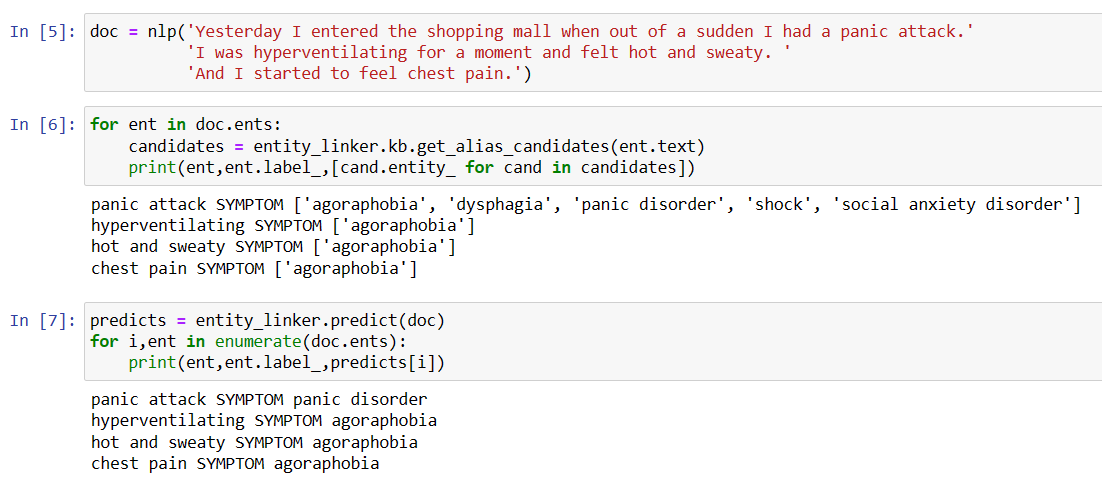
\includegraphics[width=\textwidth]{pictures/EntityLinkerDemo.png}
    \caption{Auszug aus dem Jupyter notebook \emph{entity\_linker\_demo.ipynb}}
    \label{fig:jupyter}
\end{figure}

In den meisten Fällen wird als Krankheit \emph{Agoraphobia (Platzangst)} angegeben, speziell für das Symptom \emph{panic attack} aber auch z.B. \emph{panic disorder} oder \emph{shock}. Eine einfache Auswertung könnte darin bestehen, die am häufigsten genannt Krankheit, hier also \emph{Agoraphobia} als die wahrscheinlichste Erkrankung zu betrachten, die zu der Beschreibung des Patienten passt.

Alternativ dazu verwendet das zweite Beispiel die Funktion \emph{predict()} des \emph{Entity Linkers}. Dieser Funktion wird das gesamte \emph{doc}-Objekt übergeben und für alle vom \emph{Entity Ruler} gefundenen Entitäten von \emph{predict()} eine Vorhersage der Erkrankung ausgegeben. Hier wird das durch die Beispielsätze trainierte statistische Modell des \emph{Entity Linkers} verwendet. Im Idealfall ist der \emph{Entity Linker} in der Lage kontextbezogen die wahrscheinlichste Erkrankung zu identifizieren. Die Zuordnung des Symptoms \emph{panic attack} zur Erkrankung \emph{panic disorder} ist hier sinnvoll, da eine \emph{Agoraphobia} nicht immer mit Panikattacken verbunden ist. Eine weitere Untersuchung des \emph{Entity Linkers} ist noch nicht erfolgt, da davon auszugehen ist, dass die Menge an Trainingssätzen noch nicht ausreicht, um eine zuverlässige Funktion des \emph{Entity Linkers} zu demonstrieren.

\subsection{Linguistische Analyse der Entitäten}

Die erstellte prototypische Implementierung erbringt bereits mit der reinen Vokabelanalyse zu Krankheiten und Symptomen gute Ergebnisse. Für weitergehende Untersuchungen scheint es von Vorteil, zu den Entitäten auch die entsprechenden Wortarten und ihre Funktion im jeweiligen Satz zu ermitteln, um darauf aufbauend genauere Beziehungen zwischen den Entitäten ermitteln zu können. Eine grundlegende Implementierung dieser Funktionalität steht mit der Methode \lstinline{analyze_linguistically()} zur Verfügung.

